%% Copyright 2009 Elsevier Ltd
%%
%% This file is part of the 'Elsarticle Bundle'.
%% ---------------------------------------------
%%
%% It may be distributed under the conditions of the LaTeX Project Public
%% License, either version 1.2 of this license or (at your option) any
%% later version.  The latest version of this license is in
%%    http://www.latex-project.org/lppl.txt
%% and version 1.2 or later is part of all distributions of LaTeX
%% version 1999/12/01 or later.
%%
%% The list of all files belonging to the 'Elsarticle Bundle' is
%% given in the file `manifest.txt'.
%%
%% Template article for Elsevier's document class `elsarticle'
%% with harvard style bibliographic references
%%
%% $Id: elsarticle-template-2-harv.tex 155 2009-10-08 05:35:05Z rishi $
%% $URL: http://lenova.river-valley.com/svn/elsbst/trunk/elsarticle-template-2-harv.tex $

%\documentclass[preprint,authoryear,12pt]{elsarticle}
%\documentclass[preprint,review,authoryear,12pt]{elsarticle}
\documentclass[final,authoryear,5p,times,twocolumn]{elsarticle}

%% Use the option review to obtain double line spacing
%% \documentclass[authoryear,preprint,review,12pt]{elsarticle}

%% Use the options 1p,twocolumn; 3p; 3p,twocolumn; 5p; or 5p,twocolumn
%% for a journal layout:
%% \documentclass[final,authoryear,1p,times]{elsarticle}
%% \documentclass[final,authoryear,1p,times,twocolumn]{elsarticle}
%% \documentclass[final,authoryear,3p,times]{elsarticle}
%% \documentclass[final,authoryear,3p,times,twocolumn]{elsarticle}
%% \documentclass[final,authoryear,5p,times]{elsarticle}
%% \documentclass[final,authoryear,5p,times,twocolumn]{elsarticle}

%% if you use PostScript figures in your article
%% use the graphics package for simple commands
%% \usepackage{graphics}
%% or use the graphicx package for more complicated commands
%% \usepackage{graphicx}
%% or use the epsfig package if you prefer to use the old commands
%% \usepackage{epsfig}

%% ---------------------------------------------------------------------------------------
%% My own calls to packages

\usepackage{gensymb}
\usepackage{textcomp}
\usepackage{color}
\usepackage{caption}
\usepackage{subcaption}

\usepackage{amsmath}

\usepackage{ifpdf}
\ifpdf
	\usepackage[pdftex,bookmarks=false]{hyperref}
\else
	\usepackage{graphics}
	\usepackage{graphicx}
	\usepackage{epsfig}
	\usepackage[dvipdfm,bookmarks=false]{hyperref}
\fi

\hypersetup{
    pdfpagelayout=OneColumn,
	colorlinks = true,
	urlcolor   = blue,
	citecolor  = blue,
	linkcolor  = blue
}

\urlstyle{same}

\clubpenalty=10000  % Orphan - First of paragraph left behind
\widowpenalty=10000 % Widow  - Last of paragraph sent ahead

%\usepackage{fancyvrb}
\usepackage{listings}
\definecolor{mylistingbkgd}{RGB}{255,255,220}
\definecolor{mylistingnclr}{RGB}{150,150,150}
\lstdefinestyle{output}{
	moredelim=**[is][\color{red}]{@}{@}
}
\lstdefinestyle{optional}{
	moredelim=**[is][\color{blue}\it]{@}{@}
}



%% ---------------------------------------------------------------------------------------

%% EPS figures and figure path
%\usepackage{epsfig}
%\graphicspath{{fig/}}

%% The amssymb package provides various useful mathematical symbols
\usepackage{amssymb}

%% The amsthm package provides extended theorem environments
%% \usepackage{amsthm}

%% The lineno packages adds line numbers. Start line numbering with
%% \begin{linenumbers}, end it with \end{linenumbers}. Or switch it on
%% for the whole article with \linenumbers after \end{frontmatter}.
%% \usepackage{lineno}

%% natbib.sty is loaded by default. However, natbib options can be
%% provided with \biboptions{...} command. Following options are
%% valid:

%%   round  -  round parentheses are used (default)
%%   square -  square brackets are used   [option]
%%   curly  -  curly braces are used      {option}
%%   angle  -  angle brackets are used    <option>
%%   semicolon  -  multiple citations separated by semi-colon (default)
%%   colon  - same as semicolon, an earlier confusion
%%   comma  -  separated by comma
%%   authoryear - selects author-year citations (default)
%%   numbers-  selects numerical citations
%%   super  -  numerical citations as superscripts
%%   sort   -  sorts multiple citations according to order in ref. list
%%   sort&compress   -  like sort, but also compresses numerical citations
%%   compress - compresses without sorting
%%   longnamesfirst  -  makes first citation full author list
%%
%% \biboptions{longnamesfirst,comma}

% \biboptions{}

\journal{Computers \& Geosciences}

% User defined extras:
% Earthquake macros
% -----------------

\newcommand{\dt}{$\Delta t$}
\newcommand{\vs}{$V_{\mathrm{S}}$}
\newcommand{\mathvs}{V_{\mathrm{S}}}
\newcommand{\vp}{$V_{\mathrm{P}}$}
\newcommand{\mathvp}{V_{\mathrm{P}}}
\newcommand{\vseq}[1]{$V_{\mathrm{S}}=#1$~m/s}
\newcommand{\vseqk}[1]{$V_{\mathrm{S}}=#1$~km/s}
\newcommand{\vsgeq}[1]{$V_{\mathrm{S}}\geq#1$~m/s}
\newcommand{\vsleq}[1]{$V_{\mathrm{S}}\leq#1$~m/s}
\newcommand{\vpeq}[1]{$V_{\mathrm{P}}=#1$~m/s}
\newcommand{\vsmin}{$V_{\mathrm{S}_{\min}}$}
\newcommand{\vsmineq}[1]{$V_{\mathrm{S}_{\min}}=#1$~m/s}
\newcommand{\vsminleq}[1]{$V_{\mathrm{S}_{\min}}\leq#1$~m/s}
\newcommand{\vsmingeq}[1]{$V_{\mathrm{S}_{\min}}\geq#1$~m/s}
\newcommand{\fmax}{$f_{_{\max}}$}
\newcommand{\mathfmax}{f_{_{\max}}}
\newcommand{\fmaxeq}[1]{$f_{_{\max}}=#1$~Hz}
\newcommand{\fmaxgeq}[1]{$f_{_{\max}}\geq#1$~Hz}
\newcommand{\fmaxleq}[1]{$f_{_{\max}}\leq\;$#1~Hz}
\newcommand{\eqmag}[1]{$M_{\mathrm{#1}}$}
\newcommand{\eqmageq}[2]{$M_{\mathrm{#1}}=#2$}
\newcommand{\eqmagleq}[2]{$M_{\mathrm{#1}}\leq#2$}
\newcommand{\eqmaggt}[2]{$M_{\mathrm{#1}}>#2$}
\newcommand{\tenexp}[2]{$#1\times 10^{#2}$}
\newcommand{\qs}{$Q_{\mathrm{S}}$}
\newcommand{\qp}{$Q_{\mathrm{P}}$}
\newcommand{\mathqs}{Q_{\mathrm{S}}}
\newcommand{\mathqp}{Q_{\mathrm{P}}}
\newcommand{\vsthirty}{$V_{\mathrm{S30}}$}
\newcommand{\vsthirtyeq}[1]{$V_{\mathrm{S30}}=#1$~m/s}
\newcommand{\fgeq}[1]{$f\geq#1$~Hz}
\newcommand{\fleq}[1]{$f\leq#1$~Hz}

% Math macros
\newcommand{\pepsi}{\epsilon^{p}}
\newcommand{\dpepsi}{\dot{\epsilon}^{p}}
\newcommand{\eepsi}{\epsilon^{e}}
\newcommand{\deepsi}{\dot{\epsilon}^{e}}
\newcommand{\depsi}{\dot{\epsilon}}

% Reference equations with parenthesis
% ------------------------------------

\newcommand{\refeqn}[1]{(\ref{#1})}

% Reference figures
% -----------------

\newcommand{\reffig}[1]{Fig.~\ref{#1}}
\newcommand{\refFig}[1]{Figure~\ref{#1}}

% Easy volume and area
% --------------------

\newcommand{\vdomain}[4]{#1~#4 $\times$ #2~#4 $\times$ #3~#4}
\newcommand{\adomain}[3]{#1~#3 $\times$ #2~#3}
\newcommand{\vgrid}[3]{#1 $\times$ #2 $\times$ #3}
\newcommand{\agrid}[2]{#1 $\times$ #2}


% XXXXXXXXXXXXXXXXXXXXXXXXXXXXXXXXXXXXXXXXXXXXXXXXXXXXXXXXXXXXXXXXXXXXXXXXXXXXXXXXXXXXXXXX



\begin{document}

\begin{frontmatter}

%% Title, authors and addresses

%% use the tnoteref command within \title for footnotes;
%% use the tnotetext command for the associated footnote;
%% use the fnref command within \author or \address for footnotes;
%% use the fntext command for the associated footnote;
%% use the corref command within \author for corresponding author footnotes;
%% use the cortext command for the associated footnote;
%% use the ead command for the email address,
%% and the form \ead[url] for the home page:
%%
%% \title{Title\tnoteref{label1}}
%% \tnotetext[label1]{}
%% \author{Name\corref{cor1}\fnref{label2}}
%% \ead{email address}
%% \ead[url]{home page}
%% \fntext[label2]{}
%% \cortext[cor1]{}
%% \address{Address\fnref{label3}}
%% \fntext[label3]{}


\title{The Unified Community Velocity Model Software Framework}


%% use optional labels to link authors explicitly to addresses:
%% \author[label1,label2]{<author name>}
%% \address[label1]{<address>}
%% \address[label2]{<address>}


\author[cs.usc]{Patrick Small\corref{cor1}\fnref{fn1}}
\ead{patrices@usc.edu}

\author[scec]{David Gil\corref{cor2}}
\ead{davidgil@usc.edu}

\author[scec]{Phil J. Maechling\corref{cor2}}
\ead{maechlin@usc.edu}

\author[mem]{Ricardo Taborda}
\author[scec,des.usc]{Thomas H. Jordan}
\author[anl]{Geoffrey P. Ely}
\author{Other Authors TBD}

\address[cs.usc]{Department of Computer Science, University of Southern California, Los Angeles, CA 90089, USA}
\address[scec]{Southern California Earthquake Center, 3651 Trousdale Parkway, Suite 169, Los Angeles, CA 90089, USA}
\address[mem]{Center for Earthquake Research and Information, and Department of Civil Engineering, University of Memphis, Memphis, TN 38152, USA}
\address[des.usc]{Department of Earth Sciences, University of Southern California, Los Angeles, CA 90089, USA}
\address[anl]{Leadership Computing Facility, Argonne National Laboratory, Argonne, IL 60439, USA}

\cortext[cor1]{Principal corresponding author}
\cortext[cor2]{Corresponding author}

\fntext[fn1]{This is only a tentative author line-up. Final line-up to be agreed upon by the whole group}


\begin{abstract}

This paper presents the Unified Community Velocity Model (UCVM) software framework developed by the Southern California Earthquake Center (SCEC). UCVM is a collection of software tools and application programming interfaces (APIs) designed to provide standardized access to multiple seismic velocity models used in seismology and geophysics research. Seismic velocity models are key components of current research efforts dedicated to advancing our knowledge of the Earth's crustal structure and its influence on ground response during earthquakes, including regional deep geology and local effects produced by the geometry, spatial distribution, and material composition of sediments in basins and valleys. The UCVM software framework has been designed to facilitate a broad range of research activities involving the use of seismic velocity models. Its development has been particularly useful to, and driven by, deterministic physics-based earthquake ground-motion simulation and seismic hazard analysis applications. The UCVM has been extensively used in modeling and simulation activities in southern California. Here, we describe the background that led to the development of the UCVM and its various software components and features, including examples of recent applications that use UCVM tools or output datasets in geoscience research.

\end{abstract}



\begin{keyword}
%% keywords here, in the form: keyword \sep keyword
%% MSC codes here, in the form: \MSC code \sep code
%% or \MSC[2008] code \sep code (2000 is the default)

seismic velocity models \sep 
earthquake simulation \sep 
high-performance computing \sep
meshing

\end{keyword}

\end{frontmatter}

% \linenumbers

%% main text



\section{Introduction}
\label{sec:introduction}

The quantitative understanding of the physical world is an essential goal of geoscience research. We use mathematical abstractions to represent the behavior of systems under static and dynamic conditions; and properties such as density and elastic moduli to characterize the capacity of materials to absorbe or transmit forces in stationary and transient processes. In seismology and geophysics, our understanding of physical phenomena associated to earthquakes, their genesis, and effects, depends in a good measure on our knowledge and accurate representation of the geometry and material properties of the Earth's structure, as well as on our capacity to represent the mechanical characteristics of the rupture process that takes place when a seismic fault breaks and the subsequent seismic wave propagation problem. We use stress conditions and dynamic rupture models to describe faulting processes; and seismic velocity and attenuation models, along with wave propagation principles to determine the characteristics of the ground motion.

Initial stress models and seismic velocity models are therefore at the most basic input-level in earthquake ground motion simulation. We are interested in how seismic velocity models are built and made available to geoscientists, and in particular, on how these models can help advance physics-based earthquake science. We utilize modeling approaches based on deterministic numerical techniques---such as the finite element, finite difference, or spectral element methods---to simulate the ground motion in ways that incorporate the physics of earthquake processes explicitly. That is, methods that explicitly solve the associated wave propagation problem. The use of physics-based earthquake simulation has increased considerably over the last two decades thanks to the growth---in capacity and availability---of high-performance computing (HPC) facilities and applications \citep[e.g.,][]{Aagaard_2008_BSSA2, Olsen_2009_GRL, Bielak_2010_GJI, Cui_2010_Proc}. These simulations have specific applications of great impact in seismology and earthquake engineering in aspects such as the assessment of regional seismic hazard \citep[e.g.,][]{Graves_2011_PAG}.

Recent simulations have highlighted the importance of velocity models in the accuracy of simulation results \citep[e.g.,][]{Taborda_2014_BSSA}. Numerous seismic velocity models have been built for specific regional or local structures and used in particular simulations over the years \citep[e.g.,][]{Frankel_1992_BSSA, Brocher_2008_BSSA, Graves_2008_BSSA}. The need for these models in simulation gave way to the conception of community velocity models (CVMs). CVMs are seismic velocity models that have been developed, maintained, advanced and used by a community of interested investigators. Some examples of CVMs for the regions of southern and northern California, Utah, and the central United States are those models developed by \citet{Kohler_2003_BSSA}, \citet{Suss_2003_JGR}, \citet{Brocher_2006_Proc}, \citet{Magistrale_2006_Tech}, \citet{RamirezGuzman_2012_BSSA}, and \citet{Plesch_2011_SCEC}. 

CVMs have been typically distributed in the form of datasets or collections of files, or in the form of computer programs that can dynamically operate on these datasets and files to provide information about the geometry and material properties of the crust in a particular region. However, these datasets and computer programs have not always been designed carefully from a computational perspective. In addition, recent advances in earthquake simulations, powered by the increasing capability of supercomputers, have increased significantly the computational demand placed on CVMs as input to these simulations. 

This paper presents the Unified Community Velocity Model (UCVM), a software framework designed to provide standardized and computationally efficient access to seismic velocity models, developed and maintained by the Southern California Earthquake Center (SCEC). UCVM is a collection of software tools and application programming interfaces (APIs) that facilitate the access to the material properties stored in CVMs. Although UCVM was conceived as a tool to aid physics-based earthquake ground-motion simulation and regional seismic hazard assessment, it can be and has been used in other geoscience and engineering applications. Here, we describe the development of UCVM and its various software components and features, including some for use in high-performance parallel computers, and present examples of recent applications of UCVM tools in geoscience and earthquake engineering research.



\section{Community Velocity Models}
\label{sec:cvms}

\textit{
\color{blue}
This section will present how CVMs work and the various CVMs available to the community today. It will basically explain that CVMs provide the triplets of Vs, Vp and density, and, as an example, we can expand on a description of CVM-S and CVM-H, including their variations CVM-SI and CVM-H+GTL.
}

\section{The UCVM Software Framework}\label{sec:ucvm}
The primary functionality provided by UCVM is the ability to query a wide array of community velocity models for material properties in a standard way. Once a velocity model has been successfully integrated with UCVM, the framework can be utilized to query for the primary and sheer seismic wave velocities ($Vp$, $Vs$) as well as the soil/rock density ($\rho$) at any geographic point within that model. The original model's local coordinate system and map projection are concealed behind a generic interface that instead allows queries by geographic latitude and longitude along with a vertical z-coordinate. The z-axis may be defined as either depth below the free surface or elevation relative to mean sea level.

To support this flexible query mechanism consistently across all models, UCVM includes a high-resolution digital elevation model (DEM). The DEM is synthesized from the USGS National Elevation Dataset (TODO: cite USGS NED) and the ETOPO1 Global Relief Model (TODO: cite ETOPO1). It currently spans the State of California along with portions of surrounding States. However, it may be modified to cover any arbitrary region of the Earth's surface, provided adequate resolution elevation datasets exist. An additional advantage to providing the built-in DEM is that UCVM is able to return the surface elevation at any query point in addition to the traditional $Vp$, $Vs$, and $\rho$ parameters.
\begin{figure}
\centering
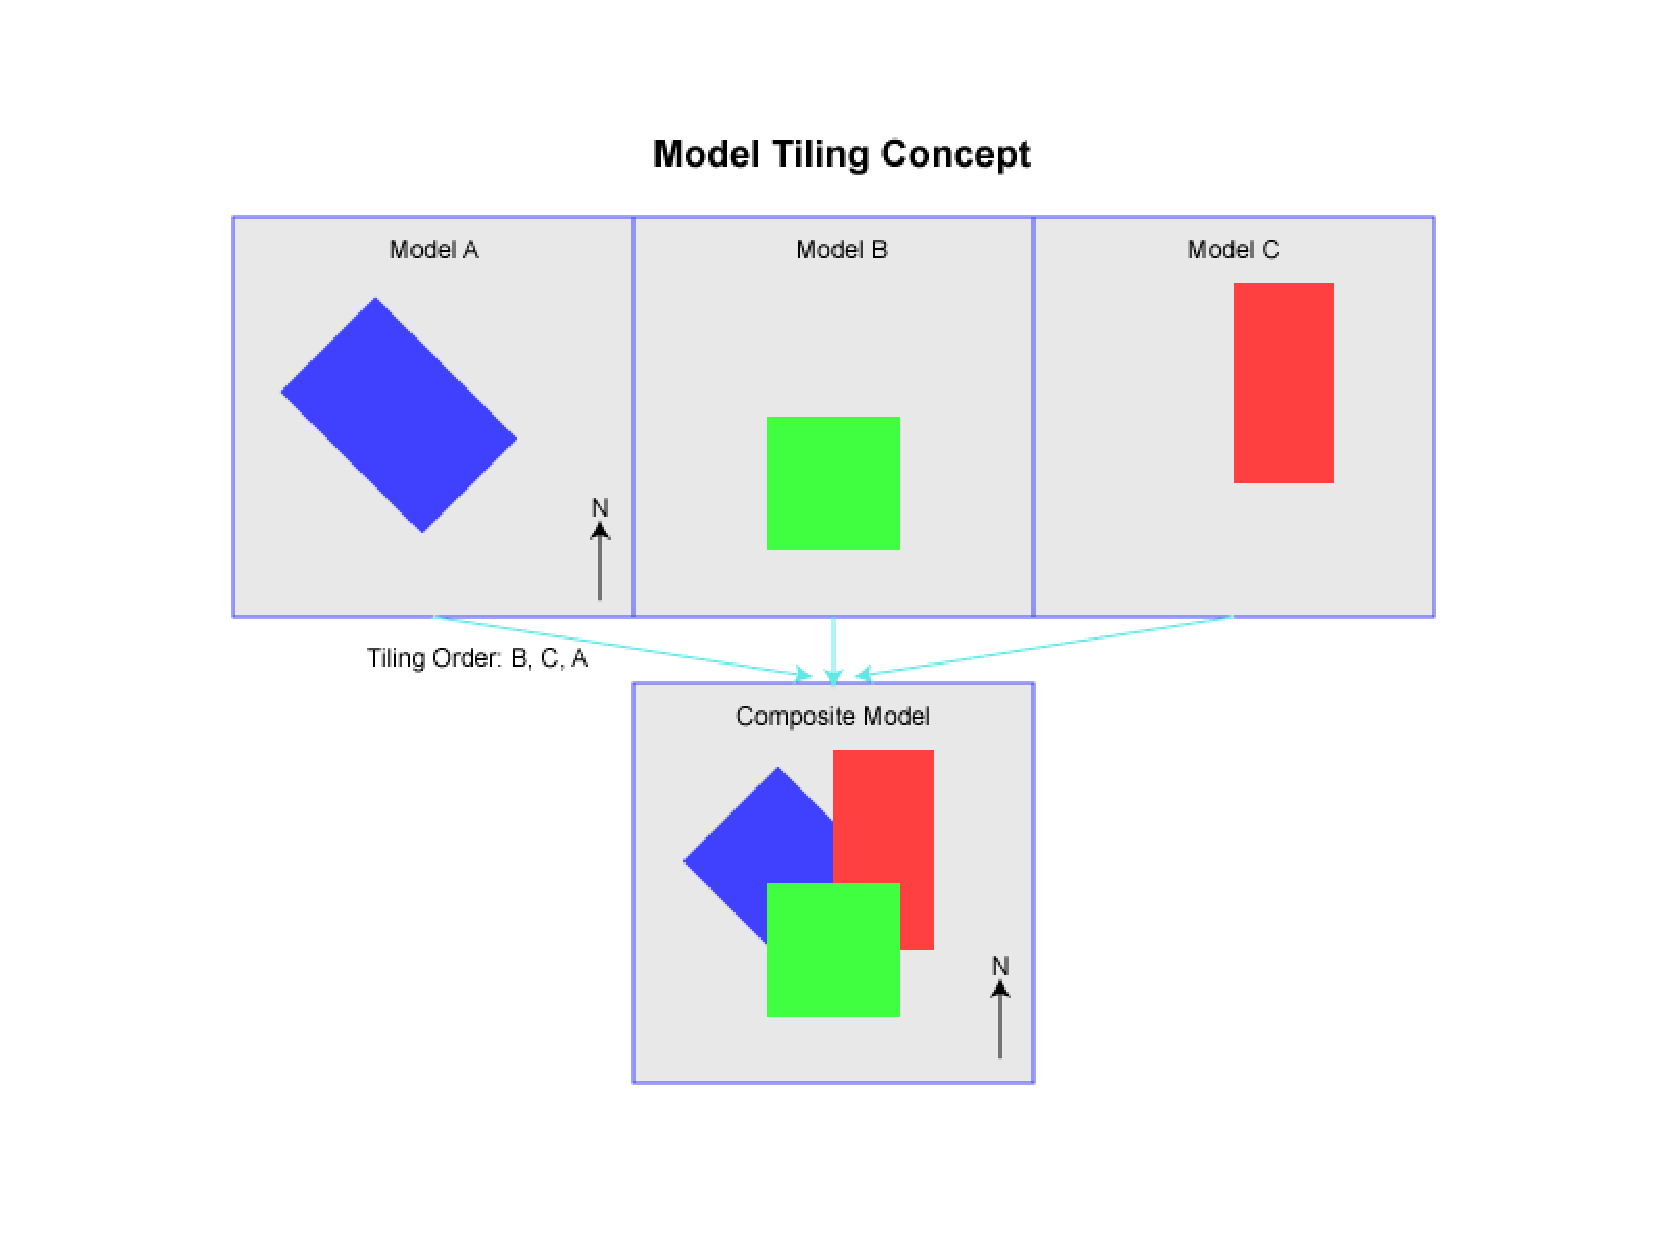
\epsfig{file=UCVM_Tiling_Concept.pdf,scale=0.35}
\caption{Tiling of velocity models (TODO: Redo/cleanup this figure).}\label{fig:tiling}
\end{figure}

The framework further extends the standardized interface by allowing multiple velocity models to be aggregated into a single composite model. Composition is accomplished by tiling two or more velocity models in three dimensions according to a user-specified priority ordering. Under this scheme, a query point is submitted sequentially to each velocity model within the ordered list that comprises the composite. The first model to return valid velocity data for the point is considered to have fulfilled the data request and subsequent models are not queried. Thus, overlap among the individual models is acceptable and their relative priority ordering arbitrates which one satisfies any given query. Generally, no smoothing is performed at the interfaces between models (an exception is interpolation between a geotechnical layer and a crustal model as discussed later in this paper). This tiling concept is illustrated in Figure \ref{fig:tiling}.

Community velocity models vary widely in their area of coverage, depth extent, and resolution. UCVM is flexible in its support for such variability. However, in order to better accommodate high frequency ground motion simulations, it categorizes models into two general groups: crustal models, and geotechnical layers (GTLs). Crustal models provide subsurface seismic wave velocities associated with basin, crust, and mantle structures. These models may potentially extend to many tens of kilometers below the Earth's surface yet do so at coarse resolutions (TODO: cite CVM-H, CVM-S). Geotechical layers, in contrast, provide velocities for only the near-surface (typically a few hundred meters) at very high resolution (TODO: cite Ely Vs30 GTL). Ground motion simulations, in particular, rely on high-resolution near-surface velocities and therefore a GTL serves to supplement the coarser data provided by crustal models.

TODO: Interpolation of GTL with Crustal

\subsection{Utilities}

\subsubsection{Querying}

\subsubsection{Gridding and Meshing}

\subsubsection{UCVM and the Etree Library}

\subsubsection{New DEMs and Vs30 Maps}

\subsection{Parallel Utilities}

\subsection{Application Programming Interface}


\section{Computational Performance}
\label{sec:conclusions}

\textit{
\color{blue}
It would be desirable to do some experiments in terms of performance, especially for the parallel applications utilities in UCVM. With some examples of how long the same thing would take if doing it differently. We will need to discuss this.
}

\section{Recent Case Applications}
\label{sec:conclusions}

\textit{
\color{blue}
This section will be dedicated to show case applications. Some ideas for potential subsections follow.
}

\subsection{Visualization and Model Comparisons}

\subsection{Chino Hills Simulation Series}

\subsection{CyberShake}

\section{Summary and Conclusions}
\label{sec:conclusions}

\textit{
\color{blue}
A couple of paragraphs with a summary of what is shown in the paper and a few key conclusions about the impact that we expect UCVM has already have and will have on earthquake research.
}



%% The Appendices part is started with the command \appendix;
%% appendix sections are then done as normal sections
%% \appendix

%% \section{}
%% \label{}

%% References
%%
%% Following citation commands can be used in the body text:
%%
%%  \citet{key}  ==>>  Jones et al. (1990)
%%  \citep{key}  ==>>  (Jones et al., 1990)
%%
%% Multiple citations as normal:
%% \citep{key1,key2}         ==>> (Jones et al., 1990; Smith, 1989)
%%                            or  (Jones et al., 1990, 1991)
%%                            or  (Jones et al., 1990a,b)
%% \cite{key} is the equivalent of \citet{key} in author-year mode
%%
%% Full author lists may be forced with \citet* or \citep*, e.g.
%%   \citep*{key}            ==>> (Jones, Baker, and Williams, 1990)
%%
%% Optional notes as:
%%   \citep[chap. 2]{key}    ==>> (Jones et al., 1990, chap. 2)
%%   \citep[e.g.,][]{key}    ==>> (e.g., Jones et al., 1990)
%%   \citep[see][pg. 34]{key}==>> (see Jones et al., 1990, pg. 34)
%%  (Note: in standard LaTeX, only one note is allowed, after the ref.
%%   Here, one note is like the standard, two make pre- and post-notes.)
%%
%%   \citealt{key}          ==>> Jones et al. 1990
%%   \citealt*{key}         ==>> Jones, Baker, and Williams 1990
%%   \citealp{key}          ==>> Jones et al., 1990
%%   \citealp*{key}         ==>> Jones, Baker, and Williams, 1990
%%
%% Additional citation possibilities
%%   \citeauthor{key}       ==>> Jones et al.
%%   \citeauthor*{key}      ==>> Jones, Baker, and Williams
%%   \citeyear{key}         ==>> 1990
%%   \citeyearpar{key}      ==>> (1990)
%%   \citetext{priv. comm.} ==>> (priv. comm.)
%%   \citenum{key}          ==>> 11 [non-superscripted]
%% Note: full author lists depends on whether the bib style supports them;
%%       if not, the abbreviated list is printed even when full requested.
%%
%% For names like della Robbia at the start of a sentence, use
%%   \Citet{dRob98}         ==>> Della Robbia (1998)
%%   \Citep{dRob98}         ==>> (Della Robbia, 1998)
%%   \Citeauthor{dRob98}    ==>> Della Robbia


%% References with bibTeX database:

\section*{References}
\bibliographystyle{model2-names}
\bibliography{references}

%% Authors are advised to submit their bibtex database files. They are
%% requested to list a bibtex style file in the manuscript if they do
%% not want to use model2-names.bst.

%% References without bibTeX database:

% \begin{thebibliography}{00}

%% \bibitem must have one of the following forms:
%%   \bibitem[Jones et al.(1990)]{key}...
%%   \bibitem[Jones et al.(1990)Jones, Baker, and Williams]{key}...
%%   \bibitem[Jones et al., 1990]{key}...
%%   \bibitem[\protect\citeauthoryear{Jones, Baker, and Williams}{Jones
%%       et al.}{1990}]{key}...
%%   \bibitem[\protect\citeauthoryear{Jones et al.}{1990}]{key}...
%%   \bibitem[\protect\astroncite{Jones et al.}{1990}]{key}...
%%   \bibitem[\protect\citename{Jones et al., }1990]{key}...
%%   \harvarditem[Jones et al.]{Jones, Baker, and Williams}{1990}{key}...
%%

% \bibitem[ ()]{}

% \end{thebibliography}

\end{document}

%%
%% End of file `elsarticle-template-2-harv.tex'.
